\chapter{\label{appendix:il2-association}}%{Association test of case-control status with pSTAT5 cell phenotype}}


% pSTAT5 MFI
\begin{figure}
\centering
\begin{minipage}{.7\textwidth}
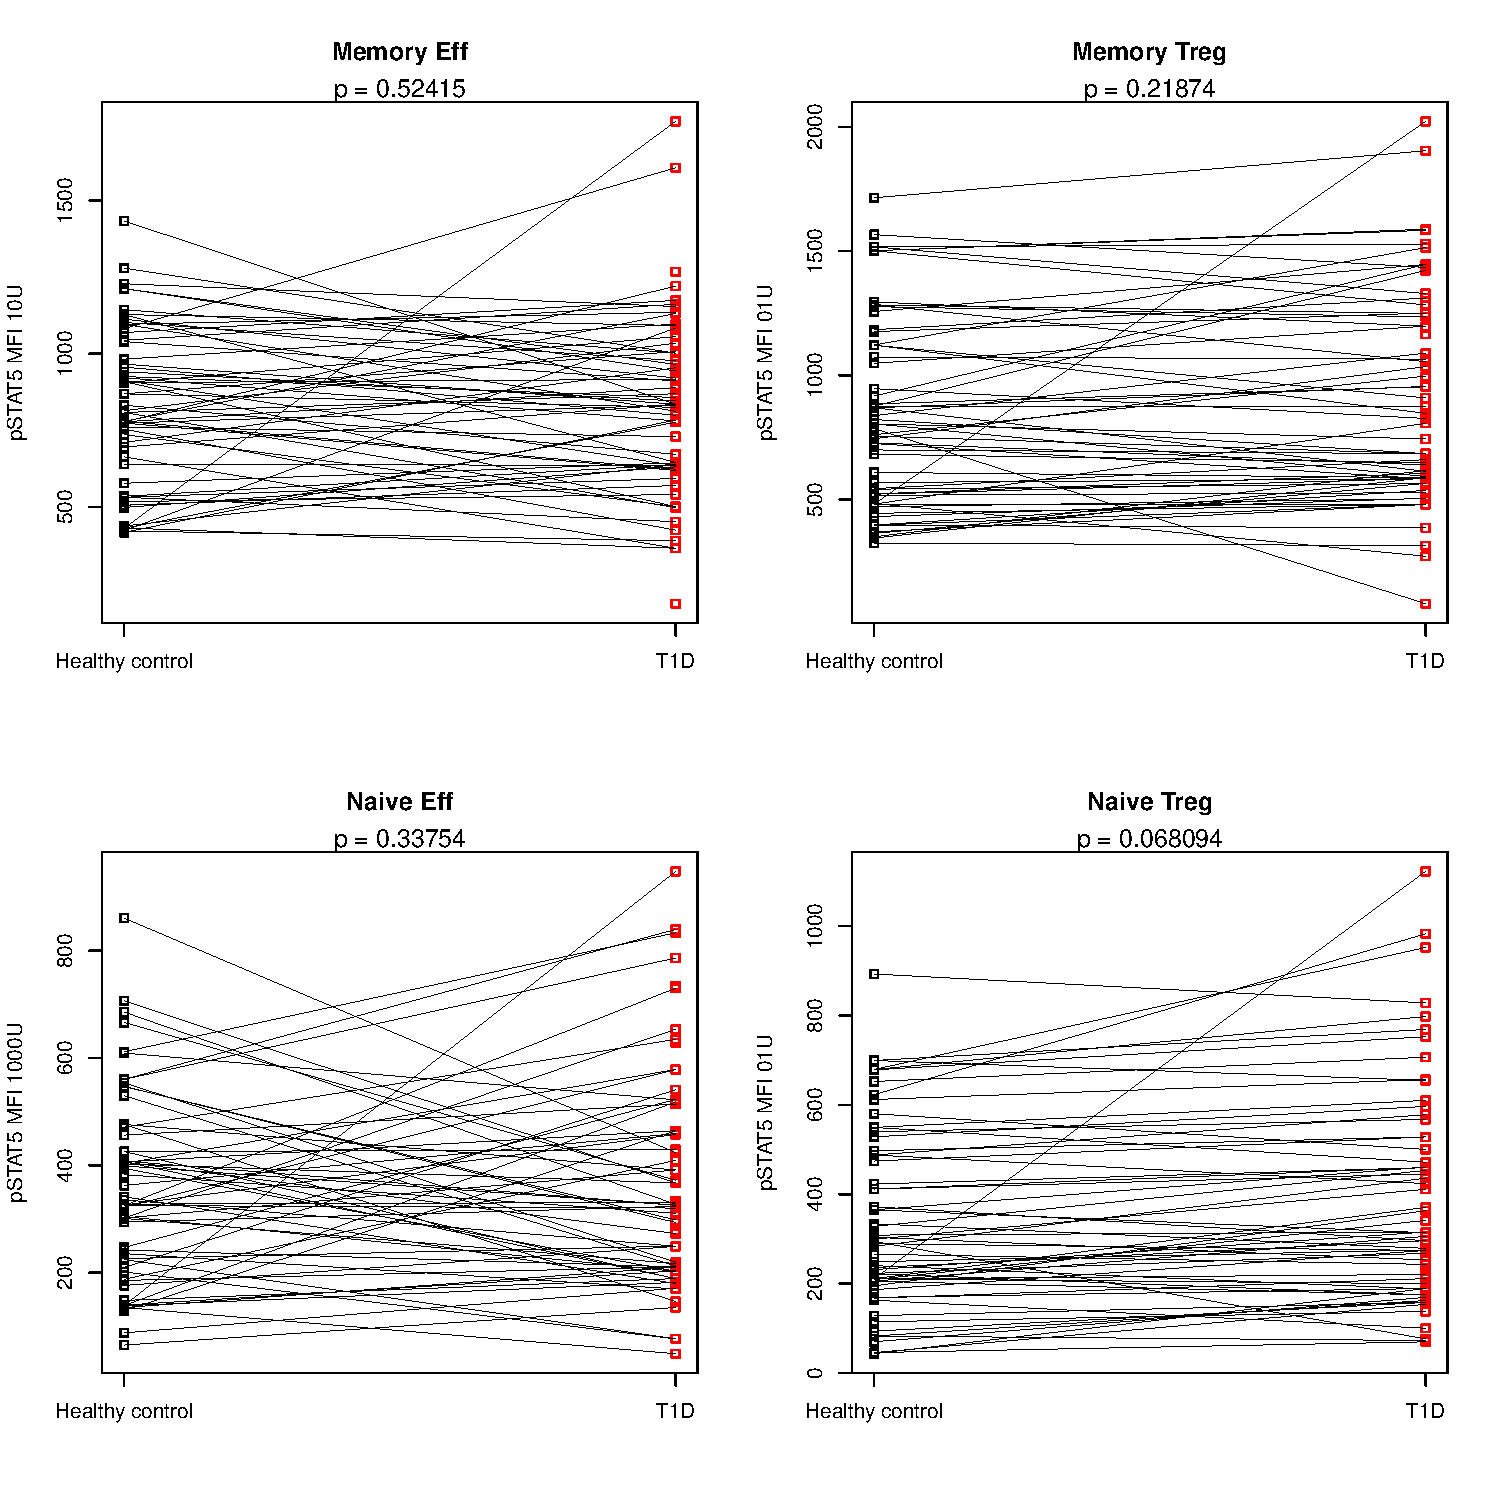
\includegraphics[width=\linewidth]{figures/pstat5-mfi-t1d-celltypes}
\end{minipage}
\mycaption{figure:pstat5-mfi-t1d-celltypes}
{ Association test of pSTAT5 MFI with T1D.  }
{
  Samples are paired by day of analysis.
  Since there are nine more cases than controls, certain cases are not paired.
}
%\end{figure}
%\begin{figure}
%\centering
\begin{minipage}{.7\textwidth}
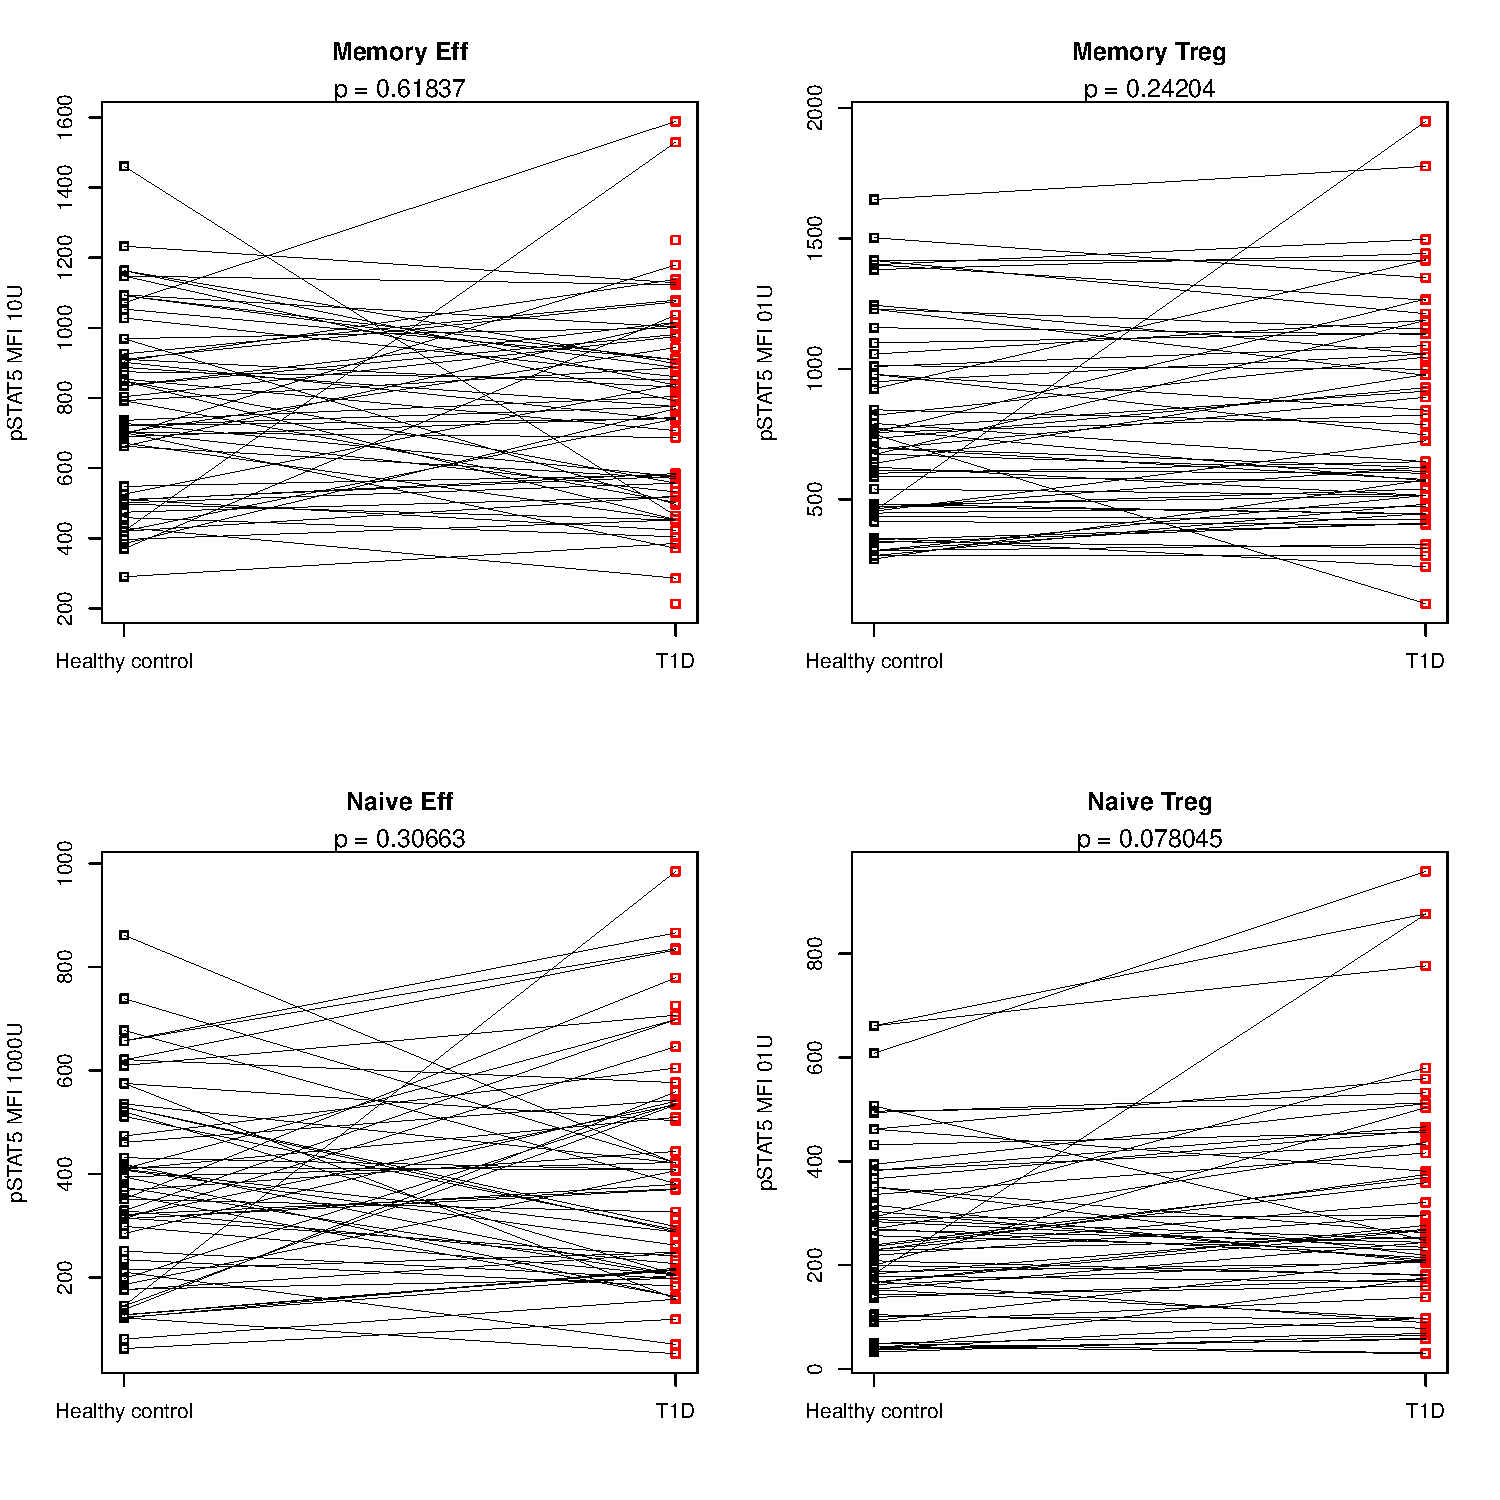
\includegraphics[width=\linewidth]{figures/nn-pstat5-mfi-t1d-celltypes}
\end{minipage}
\mycaption{figure:nn-pstat5-mfi-t1d-celltypes}
{ Association test of pSTAT5 MFI, after nearest-neighbour normalisation, with T1D.  }
{ }
{ }
\end{figure}

% pct pSTAT5+
\begin{figure}
\centering
\begin{minipage}{.7\textwidth}
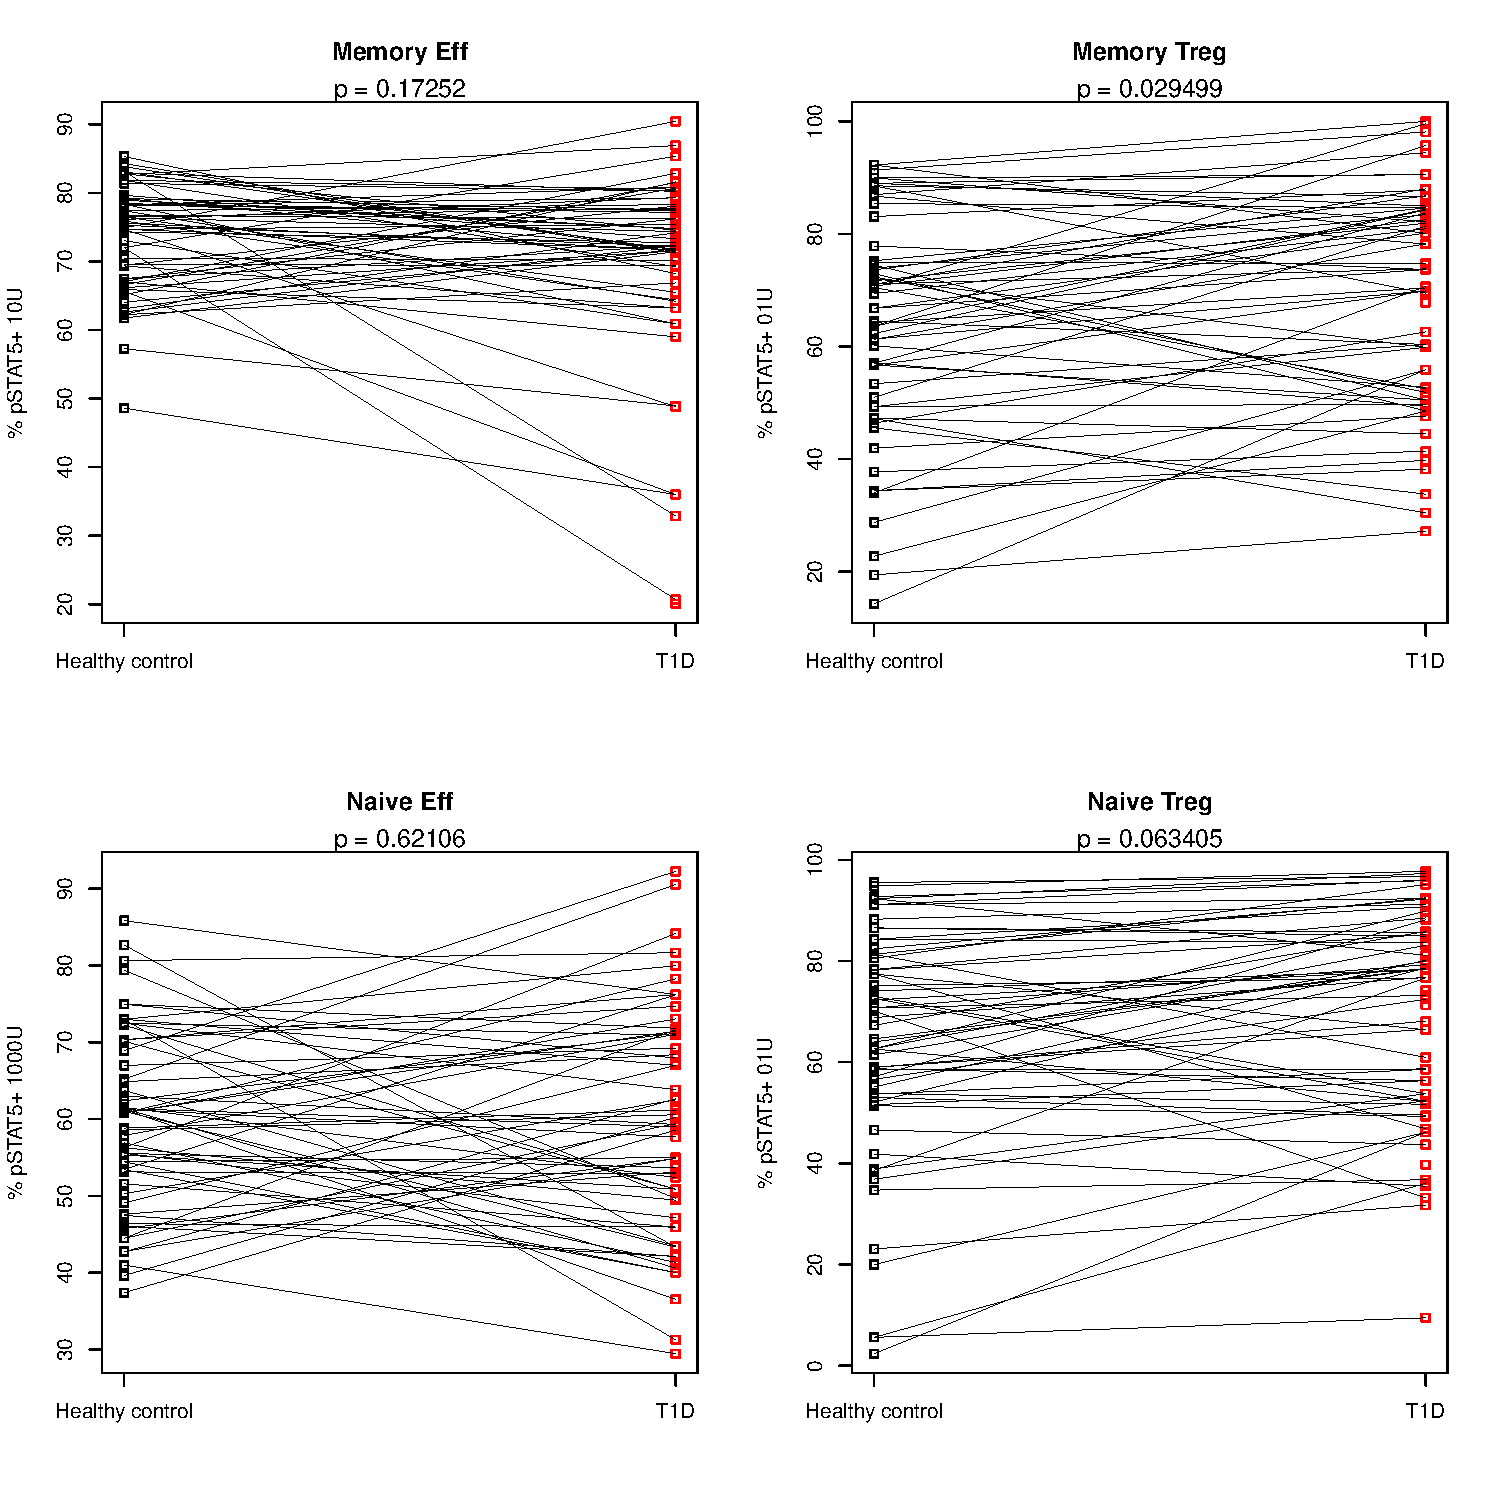
\includegraphics[width=\linewidth]{figures/pstat5-pos-t1d-celltypes}
\end{minipage}
\mycaption{figure:pstat5-pos-t1d-celltypes}
{ Association test of percent pSTAT5\positive with T1D. }
{ }
\begin{minipage}{.7\textwidth}
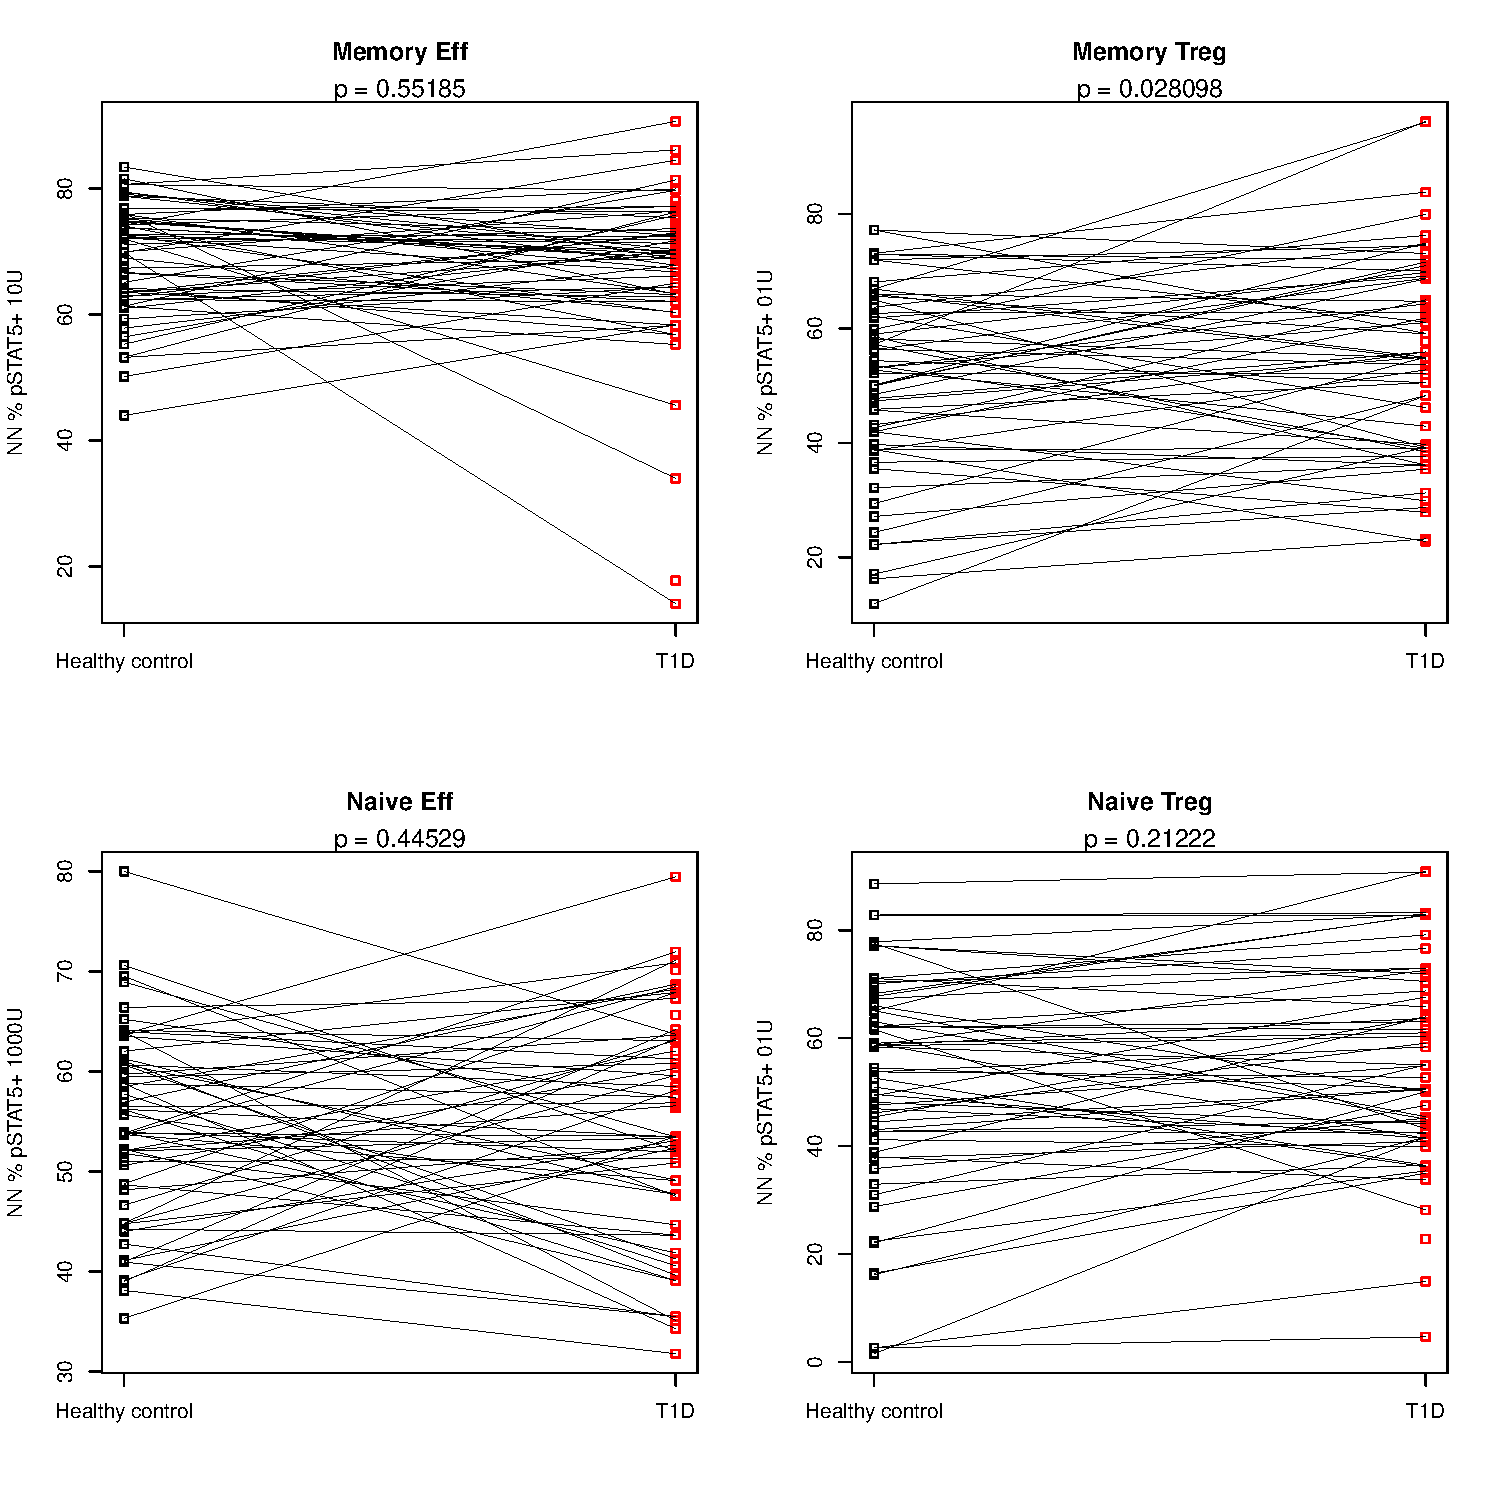
\includegraphics[width=\linewidth]{figures/nn-pstat5-pos-t1d-celltypes}
\end{minipage}
\mycaption{figure:nn-pstat5-pos-t1d-celltypes}
{ Association test of percent pSTAT5\positive, after nearest-neighbour normalisation, with T1D.  }
{ } 
\end{figure}


